\documentclass[12pt,a4paper]{article}

\usepackage{fontspec} % Пакет для работы со шрифтами в XeLaTeX
\setmainfont{Liberation Serif} % Теперь эта команда сработает
\usepackage[russian]{babel}

% Математические пакеты
\usepackage{amsmath,amssymb,amsfonts,amsthm}
\usepackage{geometry}
\geometry{top=2cm,bottom=2cm,left=3cm,right=1.5cm}

% Пакеты для оформления таблиц и графики
\usepackage{booktabs}
\usepackage{float}
\usepackage{graphicx}
\usepackage{hyperref}

% Настройка ссылок
\hypersetup{
    colorlinks=true,
    linkcolor=blue,
    filecolor=magenta,      
    urlcolor=cyan,
    pdftitle={РГР №2 - Проверка статистических гипотез},
    pdfpagemode=FullScreen,
}

\begin{document}

% % ==========================================
% % ТИТУЛЬНЫЙ ЛИСТ (Упрощенный академический стиль)
% % ==========================================
% \begin{titlepage}
%     \centering
%     \fontsize{12pt}{14pt}\selectfont
%     Министерство науки и высшего образования Российской Федерации \\
%     Федеральное государственное автономное образовательное учреждение \\
%     высшего образования «Национальный исследовательский университет ИТМО» \\
%     \vspace{4cm}
    
%     \fontsize{16pt}{18pt}\selectfont
%     \textbf{Дисциплина: Математическая статистика} \\
%     \vspace{1.5cm}
%     \fontsize{18pt}{20pt}\selectfont
%     \textbf{Расчётно-графическая работа №2} \\
%     \textbf{«Проверка статистических гипотез»} \\
%     \vspace{1cm}
%     \fontsize{14pt}{16pt}\selectfont
%     \textbf{Вариант: А--7} \\
%     \vspace{4cm}
    
%     \hfill
%     \begin{minipage}{0.5\textwidth}
%         \fontsize{12pt}{14pt}\selectfont
%         \textbf{Выполнил студен(т/ка):} \\
%         Имя Фамилия \\
%         Группа: XXXXX \\
%         \\
%         \textbf{Преподаватель:} \\
%         Смирнов И. С., Лукина М. В.
%     \end{minipage}
    
%     \vfill
%     \fontsize{12pt}{14pt}\selectfont
%     Санкт-Петербург, 2026 г.
% \end{titlepage}

\begin{titlepage}
    \centering
    \textbf{Министерство науки и высшего образования Российской Федерации}\\
    ФЕДЕРАЛЬНОЕ ГОСУДАРСТВЕННОЕ АВТОНОМНОЕ ОБ ОБРАЗОВАТЕЛЬНОЕ\\
    УЧРЕЖДЕНИЕ ВЫСШЕГО ОБРАЗОВАНИЯ\\
    \textbf{НАЦИОНАЛЬНЫЙ ИССЛЕДОВАТЕЛЬСКИЙ УНИВЕРСИТЕТ ИТМО}\\
    \vspace{1cm}
    Факультет безопасности информационных технологий\\
    \vspace{2cm}
    Дисциплина:\\
    «Математическая статистика»\\
    \vspace{2cm}
    \textbf{ОТЧЕТ ПО РАСЧЕТНО-ГРАФИЧЕСКОЙ РАБОТЕ №2}\\
    «Проверка статистических гипотез» \\
    \vspace{3cm}
    \begin{flushright}
        \textbf{Выполнили:}\\
        Пахомов Владимир Юрьевич, студент группы N3250\\
        Афанасьев Кирилл Александрович, студент группы N3251\\
        \vspace{0.5cm}
        \textbf{Проверил:}\\
        Возианова Анна Викторовна\\
    \end{flushright}
    \vfill
    Санкт-Петербург\\
    2026
\end{titlepage}

\newpage
\tableofcontents
\newpage

% ==========================================
% ВВЕДЕНИЕ / ИСХОДНЫЕ ДАННЫЕ
% ==========================================
\section{Исходные данные и описание выборки}
В рамках данной расчетно-графической работы анализируется выданный файл данных для варианта \textbf{А--7}. 
Основные характеристики исследуемой выборки приведены ниже:
\begin{itemize}
    \item \textbf{Идентификатор варианта:} А--7
    \item \textbf{Объем выборки ($n$):} 97 наблюдений для каждого столбца.
    \item \textbf{Уровень значимости ($\alpha$):} $0.05$ (используется по умолчанию для всех задач).
    \item \textbf{Исследуемые переменные:} Четыре столбца количественных данных ($X_1, X_2, X_3, X_4$).
\end{itemize}

% ==========================================
% РАЗДЕЛ 4.1: СХЕМА ПРОВЕРКИ
% ==========================================
\section{Общая схема проверки статистических гипотез (Пункт 4.1)}
Для каждого из последующих разделов проверка гипотез производится по стандартной схеме:
\begin{enumerate}
    \item \textbf{Формулировка гипотез:} задаются нулевая гипотеза $H_0$ (утверждение об отсутствии эффекта или равенстве параметру) и двусторонняя альтернативная гипотеза $H_1$ (утверждение о наличии значимого различия).
    \item \textbf{Задание уровня значимости:} фиксируется величина $\alpha = 0.05$.
    \item \textbf{Выбор критерия:} подбирается статистический критерий, исходя из структуры данных и проверяемого утверждения.
    \item \textbf{Интерпретация ошибки первого рода:} Ошибка первого рода заключается в отклонении верной нулевой гипотезы $H_0$ (риск обнаружить несуществующее различие или закономерность). Вероятность совершить данную ошибку ограничена значением $\alpha$.
    \item \textbf{Принятие статистического решения:} 
    \begin{itemize}
        \item На основе сравнения наблюдаемого значения критерия $h_{\text{набл}}$ с критической областью $W$: если $h_{\text{набл}} \in W$, то гипотеза $H_0$ отвергается.
        \item На основе $p$-value: если $p\text{-value} < \alpha$, нулевая гипотеза $H_0$ отвергается.
    \end{itemize}
\end{enumerate}

% ==========================================
% РАЗДЕЛ 4.2: СРАВНЕНИЕ СРЕДНИХ (ПАРАМЕТРИЧЕСКИЙ)
% ==========================================
\section{Проверка гипотезы о равенстве математических ожиданий для двух независимых выборок (Пункт 4.2)}

\subsection{Формулировка гипотез}
Проверяется гипотеза о равенстве средних значений генеральных совокупностей для переменных $X_1$ и $X_2$ при условии равенства дисперсий (гомоскедастичности):
\begin{align*}
    H_0 &: E(X_1) = E(X_2) \quad \text{(средние значения равны)} \\
    H_1 &: E(X_1) \neq E(X_2) \quad \text{(средние значения значимо различаются)}
\end{align*}

\subsection{Выбор критерия}
Выбран \textbf{двухвыборочный двухсторонний $t$-критерий Стьюдента} для независимых выборок с предположением о равенстве дисперсий. Применение параметрического критерия обосновано тем, что данные в столбцах $X_1$ и $X_2$ близки по структуре к непрерывным случайным величинам без экстремальных выбросов.

\subsection{Результаты расчетов}
По выборочным данным объемом $n_1 = n_2 = 97$ были получены следующие результаты вычислений:
\begin{itemize}
    \item Степени свободы: $df = n_1 + n_2 - 2 = 97 + 97 - 2 = 192$.
    \item Наблюдаемое значение статистики: $t_{\text{набл}} = 6.3024$.
    \item Критическое значение критерия для $\alpha = 0.05$: $t_{\text{крит}} = 1.9724$.
    \item Двусторонняя критическая область: $W = (-\infty, -1.9724] \cup [1.9724, +\infty)$.
    \item Достигаемый уровень значимости: $p\text{-value} = 2.0 \times 10^{-9}$.
\end{itemize}


\includegraphics[width=16cm]{graphic1.png}

\subsection{Вывод и интерпретация}
Поскольку $t_{\text{набл}} = 6.3024$ попадает в критическую область ($|t_{\text{набл}}| > 1.9724$), а полученное значение $p\text{-value} < \alpha$, нулевая гипотеза $H_0$ уверенно \textbf{отвергается}. 

\textbf{Вывод на языке исходной задачи:} Между средними значениями выборок $X_1$ и $X_2$ присутствуют статистически значимые различия на уровне значимости $5\%$. Ошибка первого рода в данной задаче заключалась бы в ложном утверждении о различии средних значений при их фактическом равенстве в генеральной совокупности.

% ==========================================
% РАЗДЕЛ 4.3: ПАРАМЕТР НОРМАЛЬНОГО РАСПРЕДЕЛЕНИЯ
% ==========================================
\section{Проверка гипотезы о параметре нормального распределения (Пункт 4.3)}

\subsection{Формулировка гипотез}
На основе карточки варианта проверяется гипотеза о равенстве математического ожидания $\mu$ переменной $X_3$ фиксированному значению $\mu_0 = 86.8$:
\begin{align*}
    H_0 &: \mu = 86.8 \\
    H_1 &: \mu \neq 86.8
\end{align*}

\subsection{Выбор критерия и результаты вычислений}
Поскольку теоретическая дисперсия $\sigma^2$ неизвестна, используется \textbf{одновыборочный $t$-критерий Стьюдента}. 
\begin{itemize}
    \item Число степеней свободы: $df = n - 1 = 96$.
    \item Наблюдаемое значение критерия: $t_{\text{набл}} = -4.0605$.
    \item Критическое значение для $\alpha = 0.05$ и $df = 96$: $t_{\text{крит}} \approx 1.9850$.
    \item Критическая область: $W = (-\infty, -1.9850] \cup [1.9850, +\infty)$.
    \item Достигаемый уровень значимости: $p\text{-value} = 0.0001$.
\end{itemize}

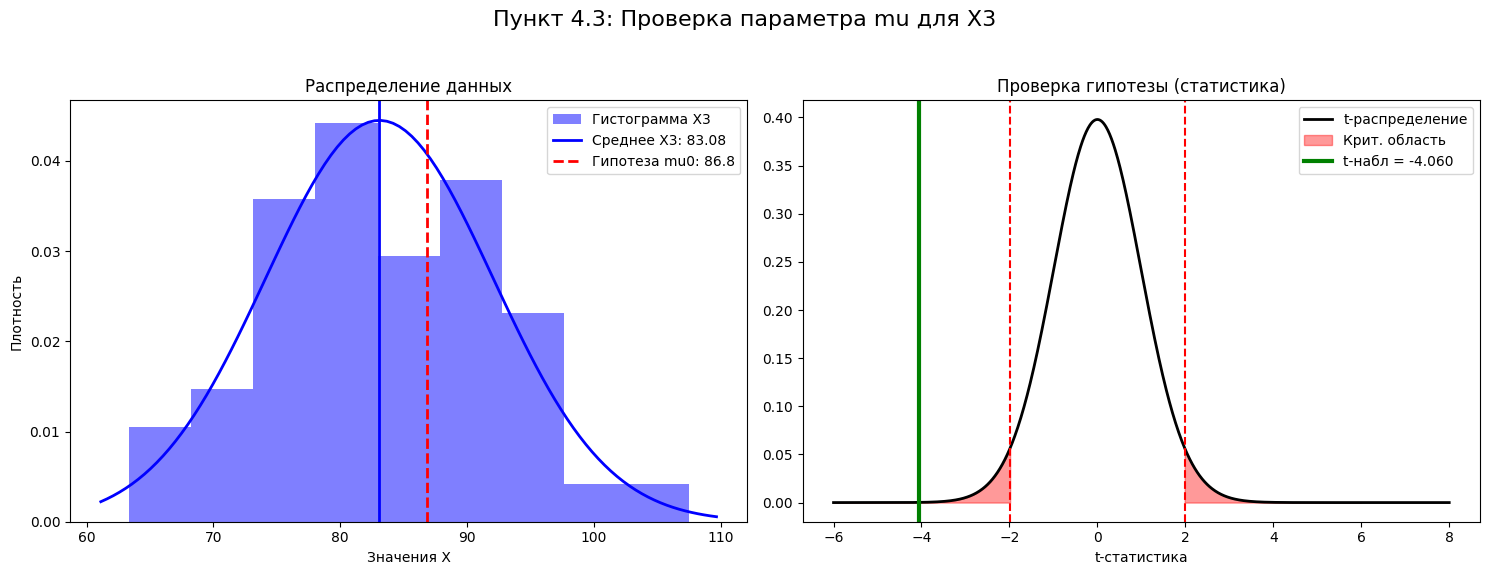
\includegraphics[width=16cm]{graphic3.png}


\subsection{Вывод и интерпретация}
Так как $|t_{\text{набл}}| = 4.0605 > 1.9850$, и полученное значение $p\text{-value} = 0.0001 < \alpha$, нулевая гипотеза $H_0$ \textbf{отвергается}. 

\textbf{Вывод на языке исходной задачи:} На основании имеющихся выборочных данных среднее значение переменной $X_3$ статистически значимо отличается от заявленного значения $86.8$. Возможная ошибка первого рода заключалась бы в ошибочном отклонении гипотезы об истинности среднего значения $\mu_0 = 86.8$.

% ==========================================
% РАЗДЕЛ 4.4: НЕПАРАМЕТРИЧЕСКИЙ КРИТЕРИЙ
% ==========================================
\section{Непараметрический критерий для двух выборок (Пункт 4.4)}

\subsection{Выбор критерия и проведение проверки}
Для сравнения двух независимых выборок $X_1$ и $X_2$ без предположения об их нормальности применен \textbf{двухвыборочный критерий Манна--Уитни} (основанный на сумме рангов наблюдений).
Гипотезы проверяются те же, что и в подразделе 4.2, но в терминах сдвига распределений.
\begin{itemize}
    \item Наблюдаемое значение статистики: $U_{\text{набл}} = 6894.0$.
    \item Достигаемый уровень значимости: $p\text{-value} < 10^{-6}$.
\end{itemize}

\subsection{Вывод и сопоставление результатов}
Поскольку полученный $p\text{-value} < \alpha$, нулевая гипотеза о равенстве законов распределения $X_1$ и $X_2$ \textbf{отвергается}. Наблюдается статистически значимый сдвиг распределений относительно друг друга.

\textbf{Сопоставление с параметрическим методом:}
Выводы параметрического критерия Стьюдента (п. 4.2) и непараметрического критерия Манна--Уитни (п. 4.4) полностью согласуются между собой. Оба метода выявили сильные систематические различия между $X_1$ и $X_2$. Такое совпадение свидетельствует о надежности полученного результата и указывает на то, что возможные отклонения данных от нормального распределения не исказили результаты классического $t$-критерия.

% ==========================================
% РАЗДЕЛ 4.5: КРИТЕРИЙ СОГЛАСИЯ ПИРСОНА
% ==========================================
\section{Критерий согласия Пирсона (Пункт 4.5)}

\subsection{Формулировка гипотез}
Проверяется гипотеза о соответствии распределения переменной $X_4$ показательному (экспоненциальному) закону с заданным параметром интенсивности $\lambda = 0.053$:
\begin{align*}
    H_0 &: X_4 \sim \text{Exp}(\lambda = 0.053) \\
    H_1 &: X_4 \text{ не соответствует данному распределению}
\end{align*}

\subsection{Методика и результаты расчетов}
Область значений выборки $X_4$ разбита на $k = 7$ интервалов согласно формуле Стерджеса. Поскольку параметр $\lambda = 0.053$ задан теоретически заранее, число степеней свободы для распределения хи-квадрат равно:
\[ df = k - 1 = 7 - 1 = 6. \]

Результаты расчета статистики критерия согласия Пирсона $\chi^2$:
\begin{itemize}
    \item Наблюдаемое значение статистики: $\chi^2_{\text{набл}} = 5.0398$.
    \item Критическое значение при $df = 6$ и $\alpha = 0.05$: $\chi^2_{\text{крит}} \approx 12.5916$.
    \item Критическая область: $W = [12.5916, +\infty)$.
    \item Полученный уровень значимости: $p\text{-value} = 0.5387$.
\end{itemize}

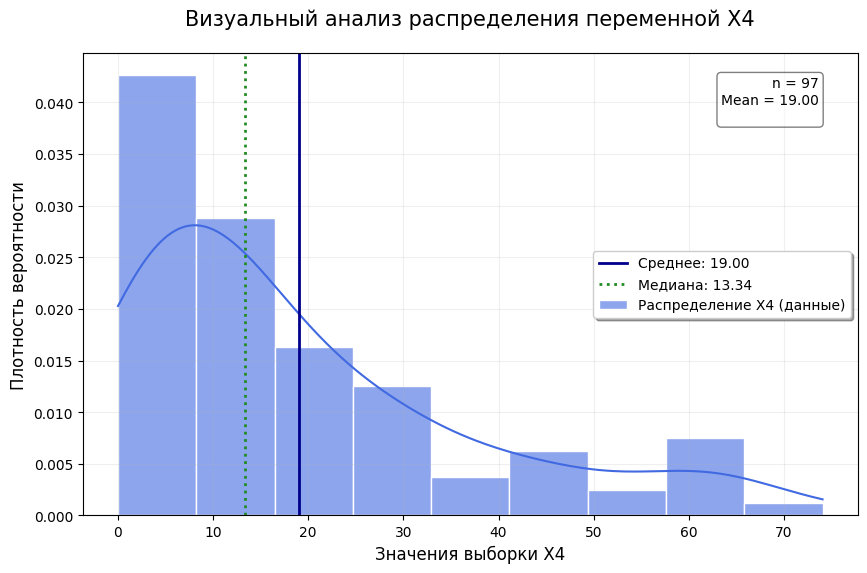
\includegraphics[width=16cm]{graphic2.png}


\subsection{Вывод и интерпретация}
Так как наблюдаемое значение статистики $\chi^2_{\text{набл}} = 5.0398$ не входит в правостороннюю критическую область ($\chi^2_{\text{набл}} < 12.5916$), а $p\text{-value} = 0.5387 > \alpha$, у нас нет статистических оснований отклонить нулевую гипотезу.

\textbf{Вывод на языке исходной задачи:} Выборочные данные переменной $X_4$ не противоречат гипотезе о том, что генеральная совокупность подчиняется показательному закону распределения с параметром интенсивности $\lambda = 0.053$. Ошибка первого рода заключалась бы в ложном отклонении согласованности теоретического закона с реальными данными.

% ==========================================
% РАЗДЕЛ 4.6: ИТОГОВЫЙ ВЫВОД
% ==========================================
\section{Итоговый вывод (Пункт 4.6)}
В процессе выполнения расчетно-графической работы №2 были применены основные методы проверки параметрических и непараметрических статистических гипотез для выборок объемом $n = 97$ (Вариант А--7):
\begin{enumerate}
    \item При сравнении средних значений двух выборок $X_1$ и $X_2$ как параметрический $t$-критерий Стьюдента ($p\text{-value} \approx 2 \times 10^{-9}$), так и непараметрический ранговый критерий Манна--Уитни ($p\text{-value} < 10^{-6}$) показали наличие статистически значимых различий на уровне значимости $0.05$. Нулевая гипотеза об однородности средних была отклонена.
    \item Проверка гипотезы о равенстве математического ожидания переменной $X_3$ фиксированному стандарту $\mu_0 = 86.8$ привела к отклонению $H_0$ ($p\text{-value} = 0.0001$).
    \item С использованием критерия согласия $\chi^2$ Пирсона проверена гипотеза о соответствии распределения $X_4$ экспоненциальному закону с интенсивностью $\lambda = 0.053$. Полученное значение $\chi^2_{\text{набл}} = 5.0398$ существенно меньше критического порога $12.5916$ ($p\text{-value} = 0.5387$), что указывает на полную согласованность опытных данных с теоретической моделью.
\end{enumerate}

\end{document}